\documentclass[12pt]{report}
\usepackage[spanish]{babel}
\usepackage[utf8]{inputenc}
\usepackage{amsmath}
\usepackage{amssymb}
\usepackage{amsthm}
\usepackage{graphics}
\usepackage{wrapfig}
\usepackage{subfigure}
\usepackage{lipsum}
\usepackage{array}
\usepackage{multicol}
\usepackage{enumerate}
\usepackage[framemethod=TikZ]{mdframed}
\usepackage[a4paper, margin = 1.5cm]{geometry}

%En esta parte se hacen redefiniciones de algunos comandos para que resulte agradable el verlos%

\renewcommand{\theenumii}{\roman{enumii}}

\def\proof{\paragraph{Demostración:\\}}
\def\endproof{\hfill$\blacksquare$}

\def\sol{\paragraph{Solución:\\}}
\def\endsol{\hfill$\square$}

%En esta parte se definen los comandos a usar dentro del documento para enlistar%

\newtheoremstyle{largebreak}
  {}% use the default space above
  {}% use the default space below
  {\normalfont}% body font
  {}% indent (0pt)
  {\bfseries}% header font
  {}% punctuation
  {\newline}% break after header
  {}% header spec

\theoremstyle{largebreak}

\newmdtheoremenv[
    leftmargin=0em,
    rightmargin=0em,
    innertopmargin=-2pt,
    innerbottommargin=8pt,
    hidealllines = true,
    roundcorner = 5pt,
    backgroundcolor = gray!60!red!30
]{exa}{Ejemplo}[section]

\newmdtheoremenv[
    leftmargin=0em,
    rightmargin=0em,
    innertopmargin=-2pt,
    innerbottommargin=8pt,
    hidealllines = true,
    roundcorner = 5pt,
    backgroundcolor = gray!50!blue!30
]{obs}{Observación}[section]

\newmdtheoremenv[
    leftmargin=0em,
    rightmargin=0em,
    innertopmargin=-2pt,
    innerbottommargin=8pt,
    rightline = false,
    leftline = false
]{theor}{Teorema}[section]

\newmdtheoremenv[
    leftmargin=0em,
    rightmargin=0em,
    innertopmargin=-2pt,
    innerbottommargin=8pt,
    rightline = false,
    leftline = false
]{propo}{Proposición}[section]

\newmdtheoremenv[
    leftmargin=0em,
    rightmargin=0em,
    innertopmargin=-2pt,
    innerbottommargin=8pt,
    rightline = false,
    leftline = false
]{cor}{Corolario}[section]

\newmdtheoremenv[
    leftmargin=0em,
    rightmargin=0em,
    innertopmargin=-2pt,
    innerbottommargin=8pt,
    rightline = false,
    leftline = false
]{lema}{Lema}[section]

\newmdtheoremenv[
    leftmargin=0em,
    rightmargin=0em,
    innertopmargin=-2pt,
    innerbottommargin=8pt,
    roundcorner=5pt,
    backgroundcolor = gray!30,
    hidealllines = true
]{mydef}{Definición}[section]

\newmdtheoremenv[
    leftmargin=0em,
    rightmargin=0em,
    innertopmargin=-2pt,
    innerbottommargin=8pt,
    roundcorner=5pt
]{excer}{Ejercicio}[section]

%En esta parte se colocan comandos que definen la forma en la que se van a escribir ciertas funciones%

\newcommand\abs[1]{\ensuremath{\left|#1\right|}}
\newcommand\divides{\ensuremath{\bigm|}}
\newcommand\cf[3]{\ensuremath{#1:#2\rightarrow#3}}
\newcommand\natint[1]{\ensuremath{\left[\!\left[ #1\right]\!\right]}}
\newcommand{\afa}{\:
    \begin{tikzpicture}
        \draw [line width = 0.17 mm, black] (0,0) -- (-0.115,0.29);
        \draw [line width = 0.17 mm, black] (0,0) -- (0.115,0.29);
        \draw [line width = 0.17 mm, black] (-0.12,0) arc (190:-10:0.12cm);
    \end{tikzpicture}
    \:
}
%Este símvolo es para casi todo salvo una cantidad finita

%recuerda usar \clearpage para hacer un salto de página

\begin{document}
    \setlength{\parskip}{5pt} % Añade 5 puntos de espacio entre párrafos
    \setlength{\parindent}{12pt} % Pone la sangría como me gusta
    \title{Un Curso Introductorio en Topología Algebraica}
    \author{Cristo Daniel Alvarado}
    \maketitle

    \tableofcontents %Con este comando se genera el índice general del libro%

    %\setcounter{chapter}{3} %En esta parte lo que se hace es cambiar la enumeración del capítulo%
    
    \chapter{Introducción}
    
    A lo largo del curso (y estudiando temas de topología) llega a resultar de útilidad analizar el siguiente problema:

    \begin{center}
        \textbf{¿Cuándo dos espacios topológicos $X$ e $Y$ son homeomorfos?}
    \end{center}

    Desafortunadamente, esta pregunta resulta en extremo compleja de analizar. Analicemos por ejemplo los siguientes subespacios de $\mathbb{R}^2$:

    %poner el ejemplo que dejó quintín en sus notas

    \chapter{El Grupo Fundamental}

    El concepto de grupo fundamental 

    \section{Conceptos Fundamentales}

    De ahora en adelante, $I$ denotará al intervalo $[0,1]$.

    \begin{mydef}
        Un \textbf{camino} o \textbf{arco} en un espacio topológico $X$, es una función continua $\cf{f}{[a,b]}{X}$ de un intervalo cerrado en $X$.

        Las imágenes $f(a)$ y $f(b)$ son llamadas \textbf{puntos finales del camino o arco}. $f(a)$ es llamado \textbf{punto inicial} y $f(b)$ \textbf{punto final}.
    \end{mydef}

    \begin{obs}
        Por comodidad, dado a que existe un homeomorfismo lineal entre $[0,1]$ y $[a,b]$ (vistos como subespacios de $\mathbb{R}$ dotado de la topología usual) siendo $a,b\in\mathbb{R}$ con $a<b$ podemos ver a todos los caminos o arcos de un espacio topológico $X$ como funciones continuas de $I$ en $X$. Cuando sea más conveniente de esta manera, se usará esta convención.
    \end{obs}

    \begin{mydef}
        Un espacio topológico $X$ es llamado \textbf{conexo por arcos} o \textbf{arco-conexo} si cualesquiera dos puntos de $X$ pueden ser unidos mediante un arco, es decir tales que los puntos finales del arco coincidan con estos dos puntos.
    \end{mydef}

    \begin{theor}
        Todo espacio topológico arco-conexo es conexo.
    \end{theor}

    \begin{proof}
        Ejercicio.
    \end{proof}

    Como una sugerencia para la demostración del teorema anterior, recuerde el \textit{teorema del cactus} (la unión de una familia de conjuntos conexos tales que la intersección de la familia es no vacía, es un conjunto conexo).

    El recíproco del teorema anterior no es cierto como se ha visto en varios cursos pasados (recuerde Cálculo III).

    \begin{mydef}
        Sea $X$ un espacio topológico. Para cada $x\in X$ se define:
        \begin{equation*}
            \mathcal{A}(x)=\left\{y\in X\Big|\textup{ existe una función continua }\cf{f}{I}{X} \textup{ tal que }f(0)=x \textup{ y }f(1)=y \right\}
        \end{equation*}
        Se construye así la familia $\left\{\mathcal{A}(x) \right\}_{ x\in X}$. Esta familia forma una partición de $X$ y se denomina como \textbf{las componentes arco-conexas de $X$}.
    \end{mydef}

    En el sentido de la definición anterior, estamos obteniendo los subconjuntos de $X$ que son arco conexos más \textit{grandes} que tiene. Si $X$ es arco-conexo, entonces $\mathcal{A}(x)=X$, para todo $x\in X$.

    Las componentes arco-conexas de $X$ no necesariamente son conjuntos cerrados o abiertos.

    \begin{mydef}
        Un espacio topológico $X$ es \textbf{localmente arco-conexo} si cada punto tiene una familia básica de vecindades arco-conexas.
    \end{mydef}

    %TODO Explicar el concepto más profundamente.

    \begin{mydef}
        Sean $\cf{f,g}{[a,b]}{X}$ dos arcos en $X$ tales que $f(a)=g(a)$ y $f(b)=g(b)$ (esto es, que ambos arcos tienen los mismos puntos terminales). Decimos que estos dos arcos son \textbf{equivalentes}, denotándolo por $f\sim g$, si existe una función continua
        \begin{equation*}
            \cf{F}{[a,b]\times I}{X}
        \end{equation*}
        tal que
        \begin{equation*}
            F(t,0)=f(t)\quad\textup{y}\quad F(t,1)=g(t)
        \end{equation*}
        para todo $t\in[a,b]$ y,
        \begin{equation*}
            F(a,s)=f(a)=g(a)\quad\textup{y}\quad F(b,s)=f(b)=g(b)
        \end{equation*}
        para todo $s\in I$.
    \end{mydef}

    \begin{propo}
        La relación de la definición anterior es una relación de equivalencia en el conjunto de todos los arcos con mismos puntos terminales de un espacio topológico $X$.
    \end{propo}

    Notemos que el concepto anterior es casi el mismo que el de homotopía, considerando de forma adicional que en esta definición se dejen fijos los puntos terminales de ambos arcos.

    \begin{mydef}
        Sean $X$ e $Y$ dos espacios topológicos. Se dice que dos funciones $\cf{f,g}{X}{Y}$ son \textbf{homotópicas} si existe una función continua $\cf{F}{X\times I}{Y}$ tal que
        \begin{equation*}
            F(x,0)=f(x)\quad\textup{y}\quad F(x,1)=g(x)
        \end{equation*}
        para todo $x\in X$.
    \end{mydef}

    \begin{obs}
        En los dos casos de las definiciones anteriores, se dota a los espacios de la topología producto.
    \end{obs}

    Intuitivamente lo que uno hace es defomar, sin perder la continuidad, un arco en el otro en el espacio $X$, dejando fijos los puntos terminales fijos en todo momento de la deformación.

    Además de esta relación inducida, queremos definir una operación para dos arcos con ciertas propiedades:

    \begin{mydef}
        Sea $X$ espacio topológico y $\cf{f}{[a,b]}{X}$ y $\cf{g}{[b,c]}{X}$ arcos tales que $f(b)=g(b)$ (siendo $a<b<c$). Entonces el producto $f\cdot g$ se define como:
        \begin{equation*}
            (f\cdot g)(t)=\left\{
                \begin{array}{lcr}
                    f(t) & \textup{ si } & t\in[a,b]\\
                    g(t) & \textup{ si } & t\in[b,c]\\
                \end{array}
            \right.
        \end{equation*}
        para todo $t\in[a,c]$.
    \end{mydef}

    \begin{obs}
        Notemos que esta operación genera otro arco, es decir otra función continua $\cf{f\cdot g}{[a,c]}{X}$.
    \end{obs}

    En lo que sigue, se usará el intervalo $I=[0,1]$.

    \section{El Grupo Fundamental de un Espacio Topológico}

    De ahora en adelante, todo camino tendrá como dominio a $I$.

    \begin{mydef}
        Sean $f$ y $g$ caminos en un espacio $X$ tales que el punto final de $f$ es el punto inicial de $g$. Se define el producto $f\cdot g$ por:
        \begin{equation*}
            f\cdot g(t)=\left\{
                \begin{array}{lcr}
                    f(2t) & \textup{ si } & 0\leq t\leq\frac{1}{2}\\
                    g(2t-1) & \textup{ si } & \frac{1}{2}\leq t\leq1\\
                \end{array}
            \right.
        \end{equation*}
        también, decimos que dos caminos $f_0$ y $f_1$ son \textbf{equivalentes} (denotado por $f_0\sim f_1$) si lo son en el sentido de la sección anterior.
    \end{mydef}

    \begin{lema}
        La relación de equivalencia y el producto definido anteriormente son compatibles en el sentido siguiente: si $X$ es un espacio, $f_0\sim f_1$ y $g_0\sim g_1$ son caminos equivalentes, entonces $f_0\cdot g_0\sim f_1\cdot g_1$ (asumiendo que el punto terminal de $f_0$ es el punto inicial de $g_0$).
    \end{lema}

    \begin{proof}
        Como el punto terminal de $f_0$ es el punto terminal de $g_0$, al tenerse las relaciones $f_0\sim f_1$ y $g_0\sim g_1$ se sigue que el producto $f_1\cdot g_1$ está bien definido.

        Como $f_0\sim f_1$ y $g_0\sim g_1$, existen dos funciones continuas $\cf{F,G}{I\times I}{X}$ tales que
        \begin{equation*}
            F(t,0)=f_0(t),\quad F(t,1)=f_1(t),\quad G(t,0)=g_0(t),\quad G(t,1)=g_1(t)
        \end{equation*}
        para todo $t\in I$, y
        \begin{equation*}
            F(0,s)=f_0(0)=f_1(0),\quad F(1,s)=f_0(1)=f_1(1)
        \end{equation*}
        y,
        \begin{equation*}
            G(0,s)=g_0(0)=g_1(0),\quad G(1,s)=g_0(1)=g_1(1)
        \end{equation*}
        para todo $s\in I$. Definamos la función $\cf{H}{I\times I}{X}$ dada por:
        \begin{equation*}
            H(t,s)=\left\{
                \begin{array}{lcr}
                    F(2t,s) & \textup{ si } & 0\leq t\leq\frac{t}{2}\\
                    G(2t-1,s) & \textup{ si } & \frac{t}{2}\leq t\leq1\\
                \end{array}
            \right.
        \end{equation*}
        para todo $t,s\in I$. Claramente $H$ es continua por el lema de pegado y dado que $F$ y $G$ son continuas, además se cumple que:
        \begin{equation*}
            \begin{split}
                H(t,0)&=\left\{
                    \begin{array}{lcr}
                        F(2t,0) & \textup{ si } & 0\leq t\leq\frac{t}{2}\\
                        G(2t-1,0) & \textup{ si } & \frac{t}{2}\leq t\leq1\\
                    \end{array}
                \right.\\
                &=\left\{
                    \begin{array}{lcr}
                        f_0(2t) & \textup{ si } & 0\leq t\leq\frac{t}{2}\\
                        g_0(2t-1) & \textup{ si } & \frac{t}{2}\leq t\leq1\\
                    \end{array}
                \right.\\
                &=f_0\cdot g_0(t)\\
            \end{split}
        \end{equation*}
        y,
        \begin{equation*}
            \begin{split}
                H(t,1)&=\left\{
                    \begin{array}{lcr}
                        F(2t,1) & \textup{ si } & 0\leq t\leq\frac{t}{2}\\
                        G(2t-1,1) & \textup{ si } & \frac{t}{2}\leq t\leq1\\
                    \end{array}
                \right.\\
                &=\left\{
                    \begin{array}{lcr}
                        f_1(2t) & \textup{ si } & 0\leq t\leq\frac{t}{2}\\
                        g_1(2t-1) & \textup{ si } & \frac{t}{2}\leq t\leq1\\
                    \end{array}
                \right.\\
                &=f_1\cdot g_1(t)\\
            \end{split}
        \end{equation*}
        para todo $t\in I$. Ademśa, para todo $s\in I$ se cumple:
        \begin{equation*}
            \begin{split}
                H(0,s)&=F(0,s)\\
                &=f_0(0)\\
                &=f_0(2\cdot0)\\
                &=f_0\cdot g_0(0)\\
            \end{split}
        \end{equation*}
        y,
        \begin{equation*}
            \begin{split}
                H(0,s)&=F(0,s)\\
                &=f_1(0)\\
                &=f_1(2\cdot0)\\
                &=f_1\cdot g_1(0)\\
            \end{split}
        \end{equation*}
        por lo cual
        \begin{equation*}
            H(0,s)=f_0\cdot g_0(0)=f_1\cdot g_1(0)
        \end{equation*}
        de forma análoga se deduce que
        \begin{equation*}
            H(1,s)=f_0\cdot g_0(1)=f_1\cdot g_1(1)
        \end{equation*}
        Se sigue de lo anterior que $f_0\cdot g_0\sim f_1\cdot g_1$.
    \end{proof}

    Como resultado de este lema, se puede definir la multiplicación de clases de equivalencia de caminos (de tal suerte que el punto terminal del primer camino coincida con el inicial del segundo camino).
    
    \begin{mydef}
        Sea $X$ espacio y $f,g$ caminos en $X$ tales que el punto terminal de $f$ es el punto inicial de $g$. $\left[f\right]$ denota a la \textbf{clase de equivalencia con representante $f$} y $\left[g\right]$ a la de $g$.

        Se define el producto de las clases $[f]$ y $[g]$ por:
        \begin{equation*}
            [f]\cdot[g]=[f\cdot g]
        \end{equation*}
    \end{mydef}

    Debido al lema anterior, el producto de clases de equivalencia está bien definido.

    Este es el tipo de multiplicación que nos va a concerner en lo que sigue. En general, la multiplicación de caminos no es asociativa.

    \begin{excer}[\textbf{La multiplicación de caminos no es asociativa.}]
        Considere en $\mathbb{R}^3$ dotado de la topología usual los caminos
        \begin{equation*}
            f(t)=(t,0,0),\quad g(t)=(0,t,0)\quad\textup{y}\quad h(t)=(0,0,t)
        \end{equation*}
        para todo $t\in I$. Compute $f\cdot (g\cdot h)$ y $(f\cdot g)\cdot h$.
    \end{excer}

    Sin embargo, se tiene el siguiente resultado:

    \begin{lema}
        La multiplicación de clases de equivalencia de caminos es asociativa.
    \end{lema}

    \begin{proof}
        Sean $f,g,h$ caminos en $X$ tales que el punto terminal de $f$ es el punto inicial de $g$ y el punto terminal de $g$ es el punto inicial de $h$. Se tiene entonces que los productos:
        \begin{equation*}
            f\cdot (g\cdot h)\quad\textup{y}\quad (f\cdot g)\cdot h
        \end{equation*}
        están bien definidos (\textit{verificar!}). Para probar el resultado, debemos ver que
        \begin{equation*}
            [f]\cdot \left([g]\cdot [h]\right)=\left([f]\cdot[g] \right)\cdot [h]
        \end{equation*}
        lo que es equivalente a probar que
        
        \begin{equation*}
            [f\cdot (g\cdot h)]=[(f\cdot g)\cdot h]
        \end{equation*}
        es decir, que $f\cdot (g\cdot h)\sim(f\cdot g)\cdot h$. Considere la función $\cf{F}{I\times I}{X}$ dada por:
        \begin{equation*}
            F(t,s)=\left\{
                \begin{array}{lcr}
                    f\left(\frac{4t}{1+s}\right) & \textup{ si } & 0\leq t\leq\frac{s+1}{4}\\
                    g(4t-1-s) & \textup{ si } & \frac{s+1}{4}\leq t\leq\frac{s+2}{4}\\
                    h\left(1-\frac{4(1-t)}{2-s}\right) & \textup{ si } & \frac{s+2}{4}\leq t\leq 1\\
                \end{array}
            \right.
        \end{equation*}

        \begin{wrapfigure}{l}{0.3\textwidth}
            \begin{center}
                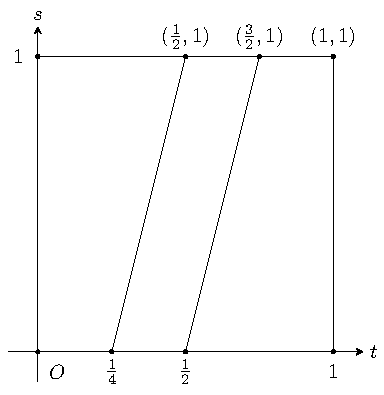
\includegraphics[scale=0.75]{images/fig_1.pdf}
            \end{center}
            \caption{Dominio de la función $F$.}
        \end{wrapfigure}

        para todo $s,t\in I$. Veamos que $F$ es continua


    \end{proof}




    \newpage

    \section{Ejercicios}

    \begin{excer}
        Pruebe que un espacio conexo y localmente arco-conexo es arco conexo.
    \end{excer}

    \begin{excer}
        Construya una deformación de retracción de $\mathbb{R}^n$ en $S^{ n-1}$.
    \end{excer}

    \begin{sol}
        
    \end{sol}

\end{document}